%##################################################
% MAGGIE
%##################################################
\section{MAGGIE}
\bartchapterimage{heic1302a_small.jpg}
\bartthumb{thumbs/heic1302a.png}

\subsection{Introduction}
\begin{frame}
    \frametitle{MAGGIE}
    \begin{block}{Models and Algorithms for Galaxy Groups, Interlopers
        and Environment}
        \begin{enumerate}
            \item<1-> Bayesian and probabilistic
            \item<2-> Better models than previous algorithms
            \item<3-> Works on doubly complete galaxy sample
        \end{enumerate}
    \end{block}
\end{frame}

\subsection{Description}
\begin{frame}
    \begin{columns}
        \begin{column}{0.4\textwidth}
            \begin{tikzpicture}[scale=0.4]
                \tikzstyle{dots}=[
                    draw,
                    shape=circle,
                    fill=black,
                    text=white,
                    scale=0.5,
                ]
                \tikzstyle{searched}=[line width=1.5pt, blue!90!white]
                \tikzstyle{linked}=[line width=2pt]

                \node[dots, visible on=<1->] (1) at (0, 1) {};
                \node[dots, visible on=<1->] (2) at (1, 2) {};
                \node[dots, visible on=<1->] (3) at (3, 4) {};
                \node[dots, visible on=<1->] (4) at (4, 7) {};
                \node[dots, visible on=<1->] (5) at (3, 6) {};
                \node[dots, visible on=<1->] (6) at (8, 4) {};
                \node[dots, visible on=<1->] (7) at (7, 3) {};
                \node[dots, visible on=<1->] (8) at (10, 1) {};
                \node[dots, visible on=<1->] (9) at (1, 10) {};
                \node[dots, visible on=<1->] (10) at (6, 1) {};
                \node[dots, visible on=<1->] (11) at (8, 3) {};
                \node[dots, visible on=<1->] (12) at (0, 4) {};
                \node[dots, visible on=<1->] (13) at (1, 8) {};
                \node[dots, visible on=<1->] (14) at (6, 2) {};
                \node[dots, visible on=<1->] (15) at (8, 8) {};
                \node[dots, visible on=<1->] (16) at (7, 6) {};
                \node[dots, visible on=<1->] (17) at (9, 9) {};
                \node[dots, visible on=<1->] (18) at (5, 5) {};
                \node[dots, visible on=<1->] (19) at (6, 4) {};

                \node[right, visible on=<2->] at (1) {8};
                \node[right, visible on=<2->] at (2) {12};
                \node[right, visible on=<2->] at (3) {9};
                \node[right, visible on=<2->] at (4) {11};
                \node[right, visible on=<2->] at (5) {10};
                \node[right, visible on=<2->] at (6) {16};
                \node[right, visible on=<2->] at (7) {6};
                \node[right, visible on=<2->] at (8) {18};
                \node[right, visible on=<2->] at (9) {5};
                \node[right, visible on=<2->] at (10) {7};
                \node[right, visible on=<2->] at (11) {2};
                \node[right, visible on=<2->] at (12) {4};
                \node[right, visible on=<2->] at (13) {15};
                \node[right, visible on=<2->] at (14) {3};
                \node[right, visible on=<2->] at (15) {14};
                \node[right, visible on=<2->] at (16) {13};
                \node[right, visible on=<2->] at (17) {17};
                \node[right, visible on=<2->] at (18) {1};
                \node[right, visible on=<2->] at (19) {19};

                \draw[searched, visible on=<3-4>] (18) circle (3);
                \draw[searched, dashed, visible on=<4>] (18) circle (2.6);

                \node[dots, fill=blue, visible on=<3->] at (19) {};
                \node[dots, fill=blue, visible on=<3->] at (18) {};
                \node[dots, fill=blue, visible on=<3->] at (16) {};
                \node[dots, fill=blue, visible on=<3->] at (4) {};
                \node[dots, fill=blue, visible on=<3->] at (3) {};
                \node[dots, fill=blue, visible on=<3->] at (5) {};

                \draw[searched, green, visible on=<5>] (11) circle (2.6);
                \draw[searched, dashed, green, visible on=<5>] (11) circle (2.3);

                \node[dots, fill=green, visible on=<6->] at (11) {};
                \node[dots, fill=green, visible on=<6->] at (6) {};
                \node[dots, fill=green, visible on=<6->] at (7) {};
                \node[dots, fill=green, visible on=<6->] at (14) {};
                \begin{scope}
                    \clip (6, 3) rectangle (7, 5);
                    \node[dots, fill=green, visible on=<6->] at (19) {};
                \end{scope}

            \end{tikzpicture}
        \end{column}
        \begin{column}{0.6\textwidth}
            \begin{block}{}
                \small
                \begin{enumerate}
                    \item<2-> Order by decreasing stellar mass or luminosity
                    \item<3-> Estimate virial radius of the group by relation
                        between central stellar mass or luminosity and the
                        dynamical mass
                    \item<4-> Compute probabilities for galaxies in virial cone and
                        keep only when $>p_\mathrm{mem}$
                    \item<5-> Loop to following galaxy if doesn't already have
                        $p>p_\mathrm{cen}$
                    \item<7-> Abundance matching between central stellar mass or
                        luminosity function and a theoretical halo mass function
                \end{enumerate}
            \end{block}
        \end{column}
    \end{columns}
\end{frame}

% \begin{frame}
    % \begin{columns}
        % \begin{column}{0.5\textwidth}
            % 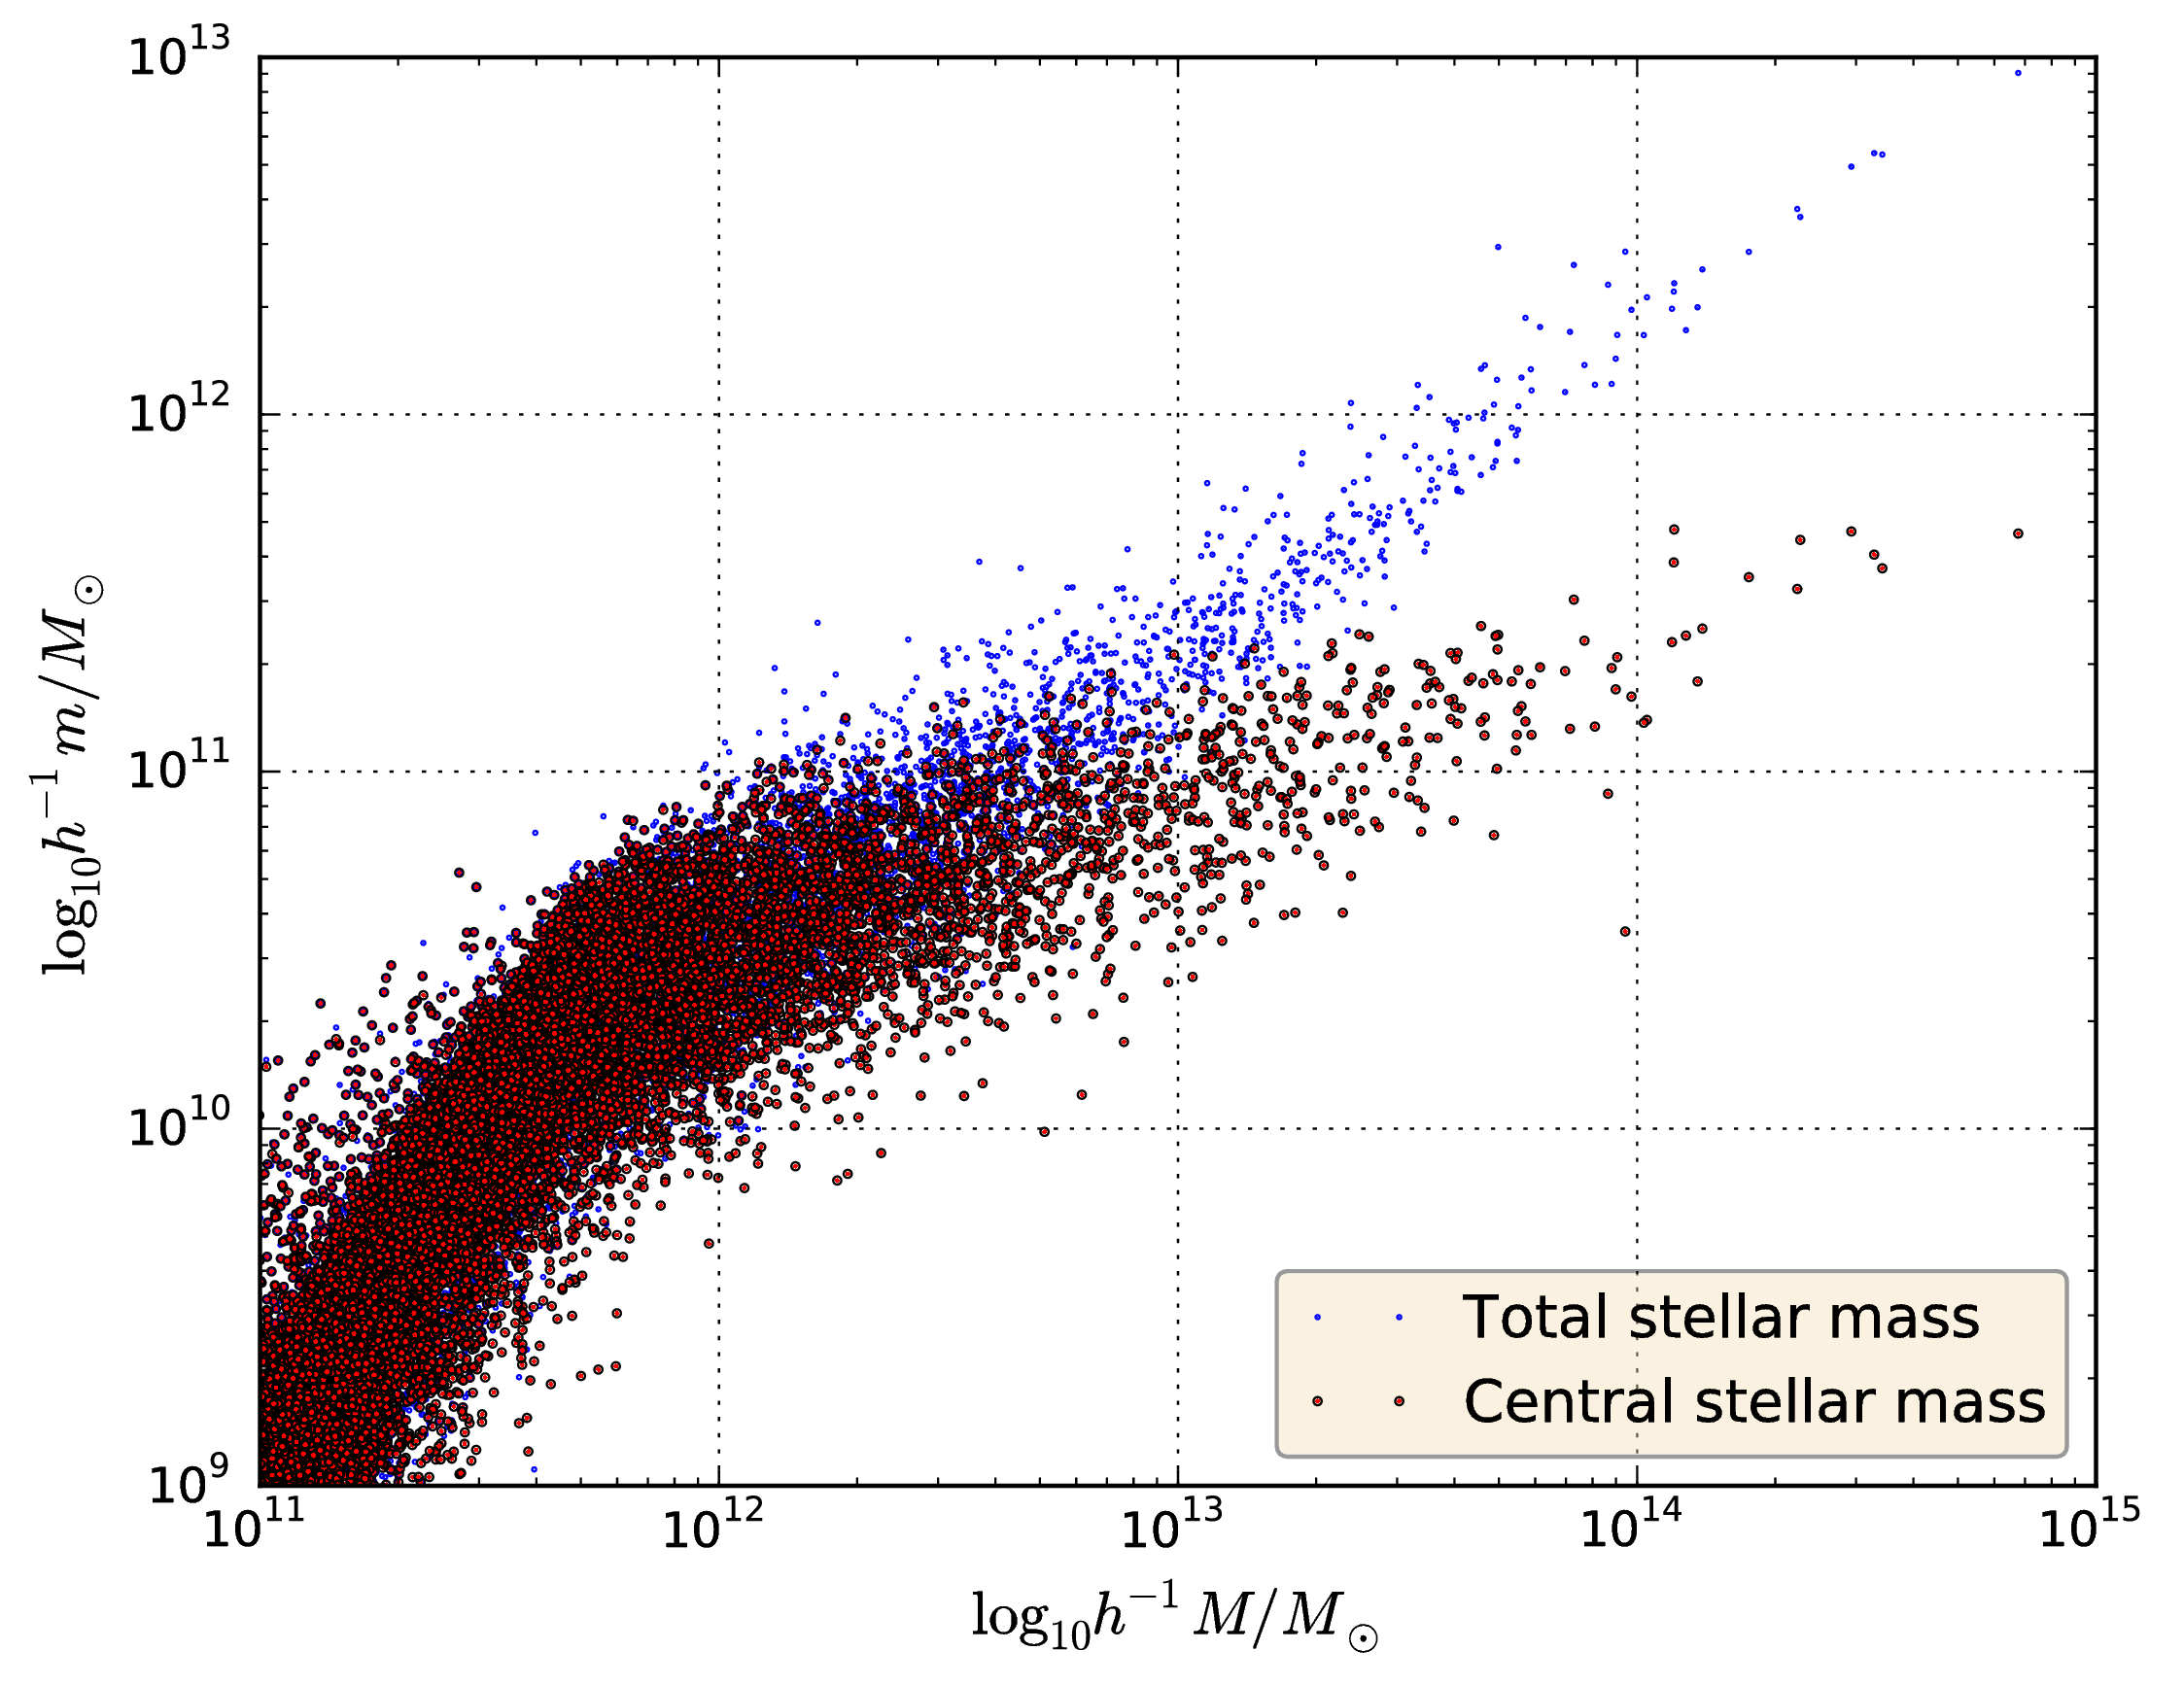
\includegraphics[width=\linewidth]{AM.png}
        % \end{column}
        % \begin{column}{0.5\textwidth}
            % \begin{block}{Abundance matching}
                % \begin{itemize}
                    % \item<1-> Central stellar mass used instead of total stellar
                        % mass
                    % \item<2-> But total stellar mass more precise than central
                    % \item<3-> But total stellar mass less efficient because we need
                        % a prior in the membership of the group
                % \end{itemize}
            % \end{block}
        % \end{column}
    % \end{columns}
% \end{frame}

\begin{frame}
    \begin{columns}
        \begin{column}{0.6\textwidth}
            \begin{block}{}
                \begin{enumerate}
                    \item<1-> Halo PPS density $g_h$: NFW density profile and
                        Gaussian 3D velocity distribution
                    \item<2-> Interloper PPS density $g_i$: from cosmological
                        simulation
                    \item<3-> Probability: ratio between PPS density of
                        galaxies in the group and total PPS density of
                        galaxies:
                        \begin{equation}
                            p\left(R, v_z\right) = \cfrac{%
                                g_h\left(R, v_z\right)
                            }{g_h\left(R, v_z\right) + g_i\left(R, v_z\right)}
                            \nonumber
                        \end{equation}
                \end{enumerate}
            \end{block}
        \end{column}
        \begin{column}{0.5\textwidth}
            \centering
            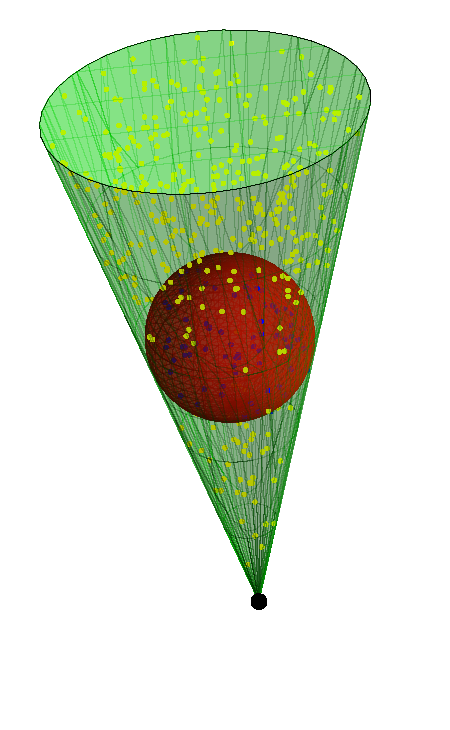
\includegraphics[width=.6\linewidth, angle=-90]{cone.pdf}\hfill
            \visible<4->{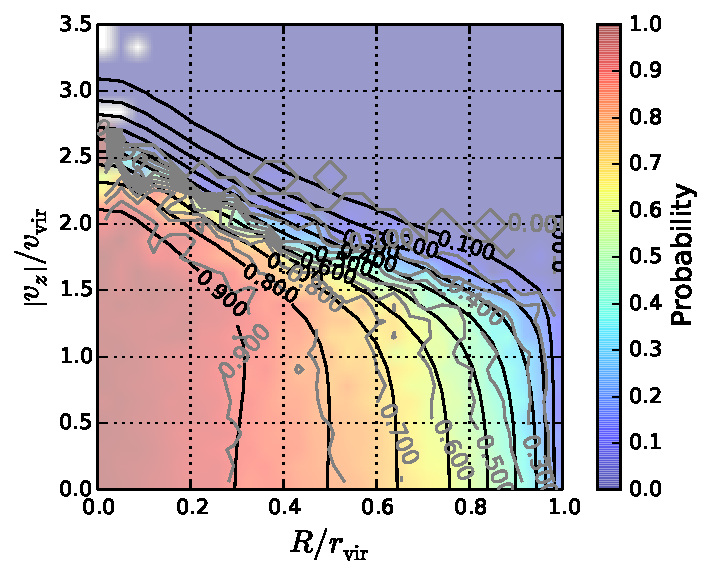
\includegraphics[width=\linewidth]{probabilities.pdf}}
        \end{column}
    \end{columns}
\end{frame}

\subsection{Results}

\begin{frame}
    \frametitle{Results}
    \begin{block}{New test definition}
        \begin{itemize}
            \item<1-> Probabilistic reliability%: $R=\cfrac{\sum_{i\in TG\cap
                % EG}p_i}{\sum_{i\in EG}p_i}$
            \item<2-> Merging not considered
        \end{itemize}
    \end{block}
\end{frame}

\newcommand\toorigin[1]{%
    ($ (current page.north west) + (\paperwidth - 3cm, -2.2) + #1 $)
}
\newcommand\legend{%
    \tikzstyle{leg}=[right, scale=0.7]
    \begin{tikzpicture}[overlay, remember picture]
        \draw[line width=2pt, blue] \toorigin{(0, 0)} -- \toorigin{(1, 0)}
            node[leg] {FoF};
        \draw[line width=2pt, green!60!black] \toorigin{(0, -0.5)} --
            \toorigin{(1, -0.5)} node[leg] {MAGGIE};
        % \draw[line width=2pt, cyan] \toorigin{(0, -1)} -- \toorigin{(1, -1)}
            % node[leg] {MAGGIE errors};
    \end{tikzpicture}
}
\begin{frame}
    \frametitle{Results}
    \framesubtitle{Fragmentation}
    \centering
    \legend%
    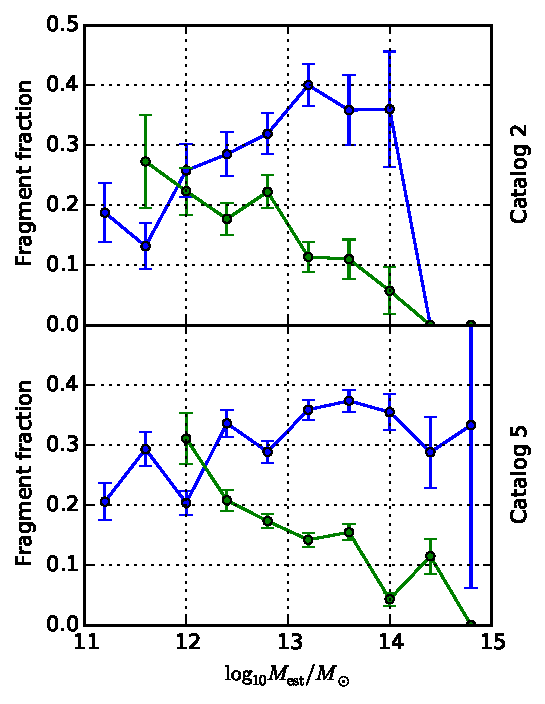
\includegraphics[height=0.6\textheight]{fragmentation.pdf}
\end{frame}

\begin{frame}
    \frametitle{Results}
    \framesubtitle{Completeness and reliability}
    \centering
    \legend%
    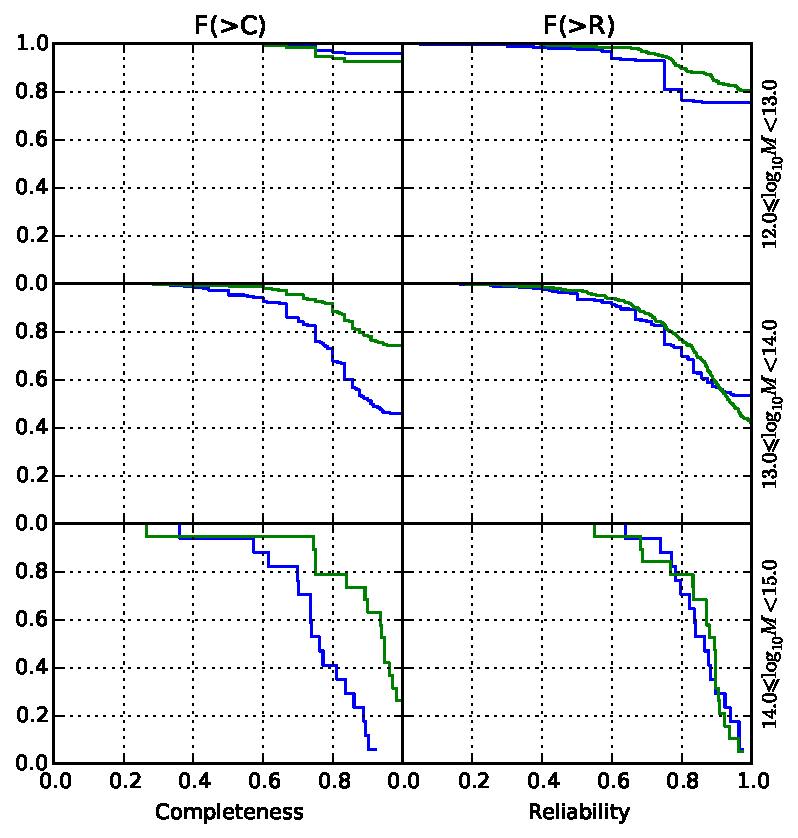
\includegraphics[height=0.6\textheight]{completeness.pdf}
\end{frame}

% \begin{frame}
    % \frametitle{Results}
    % \framesubtitle{Group stellar masses and luminosities}
    % \legend%
    % \begin{columns}
        % \begin{column}{0.55\linewidth}
            % 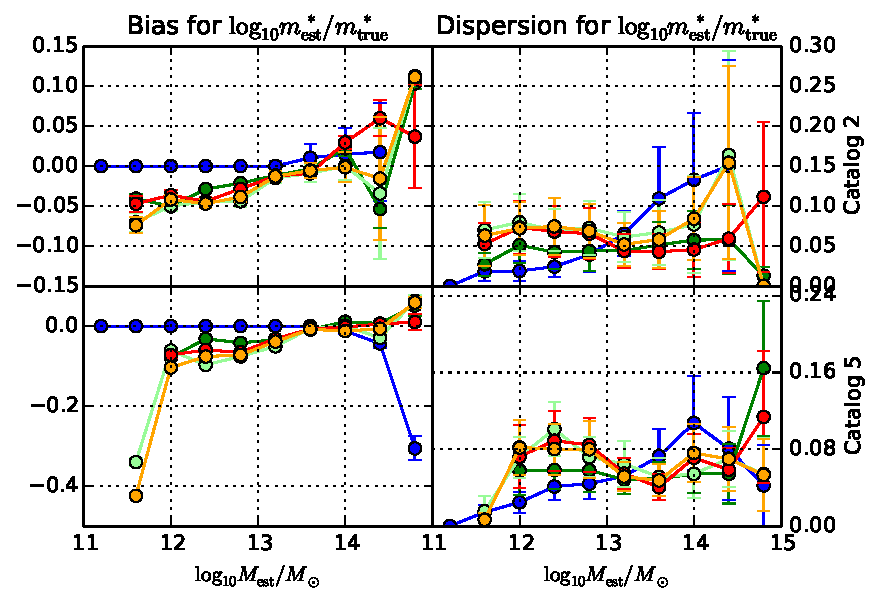
\includegraphics[width=\linewidth]{stellarmasses.pdf}
        % \end{column}
        % \begin{column}{0.55\linewidth}
            % 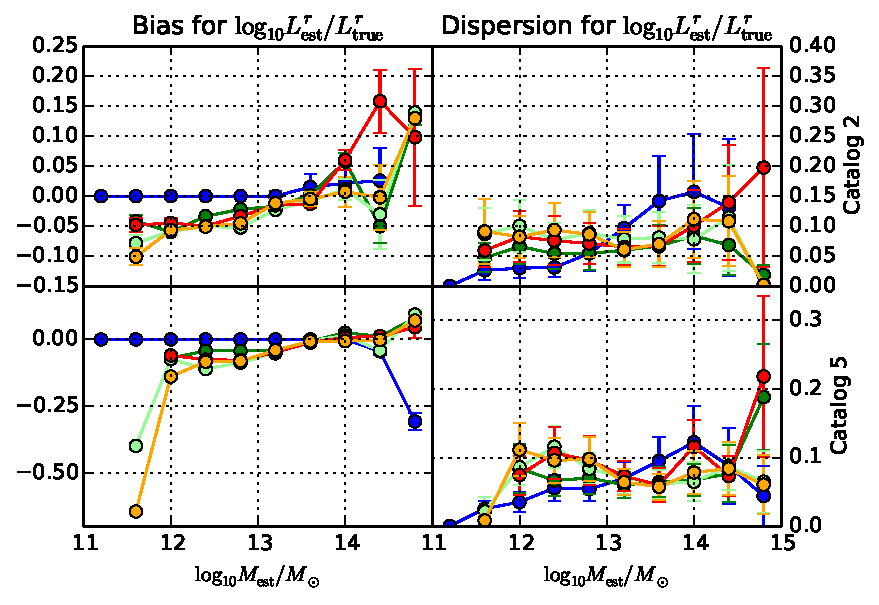
\includegraphics[width=\linewidth]{luminosities.pdf}
        % \end{column}
    % \end{columns}
% \end{frame}

\begin{frame}
    \frametitle{Results}
    \framesubtitle{Halo masses}
    \centering
    \legend%
    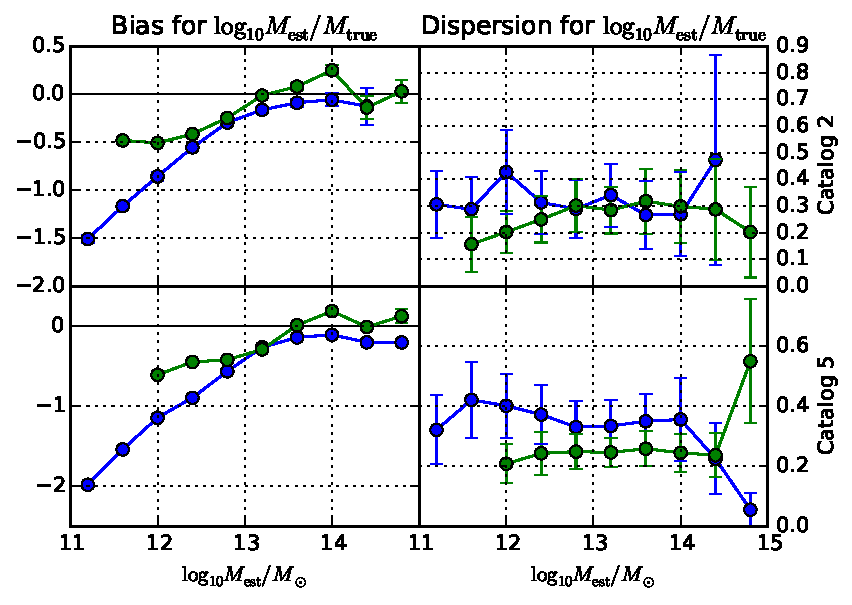
\includegraphics[height=0.6\textheight]{halomass.pdf}
\end{frame}

\begin{frame}
    \frametitle{Results}
    \framesubtitle{Robustness}
    \begin{block}{Robust against}
        \begin{enumerate}
            \item<1-> Choice of priors (initial virial mass relation, halo
                concentration)
            \item<2-> Choice of the cosmology
            \item<3-> Choice of the halo mass function
            \item<4-> Observational errors (stellar masses, luminosities, etc)
        \end{enumerate}
    \end{block}
\end{frame}


% vim: set tw=79:
